% !TEX root = ../../../main.tex
% 来源：中学数学实验教材·第一册（代数）
% 章节：多项式的四则运算 / 一元多项式的除法
% 原始文件：4.tex，行 1889-1909
% 类型：tikz
% ---
    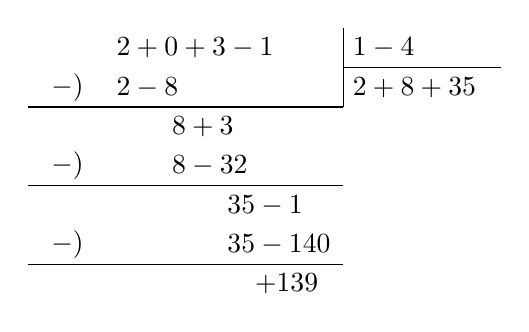
\begin{tikzpicture}
       \node at (0,.5) [right]{$2+0+3-1$};   
       \node at (0,0) [right]{$2-8$}; 
       \node at (0,-.5) [right]{\qquad $8+3$}; 
       \node at (0,-1) [right]{\qquad $8-32$}; 
       \node at (0,-1.5) [right]{\qquad \qquad $35-1$}; 
       \node at (0,-2) [right]{\qquad\qquad $35-140$}; 
      \node at (0,-2.5)[right]{\quad\qquad\qquad $+139$};
      
      \foreach \x in {-.25,-1.25,-2.25}
      {
          \draw (-1, \x)--(3,\x);
          \node at (-.5, \x+.25){$-)$};
      }
      
      \draw (3,.75)--(3,-.25);
      \draw (3,.25)--(5,.25);
      \node at (3,.5)[right]{$1-4$};
      \node at (3,0) [right]{$2+8+35$};
      
      \end{tikzpicture}
